\documentclass[11pt]{article}
\usepackage[utf8]{inputenc}
\usepackage[T1]{fontenc}
\usepackage[margin=0.85in]{geometry}
\usepackage{amsmath,amssymb,amsthm}
\usepackage{booktabs}
\usepackage{array}
\usepackage{url}
\usepackage{microtype}
\usepackage{graphicx}
\usepackage{caption}
\usepackage{xcolor}
\usepackage{listings}
\usepackage{seqsplit}
\newcommand{\hash}[1]{{\ttfamily\expandafter\seqsplit\expandafter{#1}}}
\usepackage[hidelinks]{hyperref}
\makeatletter\g@addto@macro{\UrlBreaks}{\do\_\do\.\do\/}\makeatother
\emergencystretch=3em
\tolerance=2000
% generated by gen_numbers.py; do not edit
\newcommand{\AllGates}{all pass}
\newcommand{\CthreeGapAbs}{3.2\times10^{-7}}
\newcommand{\CthreeMax}{0.995}
\newcommand{\CtlRc}{0}
\newcommand{\CtlSha}{7a3904240f4734df1360471af1bce7fb420ff279298298da6effc9f5c9e065ce}
\newcommand{\CtwoGapRel}{5.2\times10^{-7}}
\newcommand{\CtwoLogSteps}{1.18, 1.10, 1.05, 1.03}
\newcommand{\CtwoTen}{1004.4}
\newcommand{\DecHtwoFour}{8.2\times10^{-10}}
\newcommand{\DecHtwoSix}{9.9\times10^{-11}}
\newcommand{\DecOmegaFour}{19.4}
\newcommand{\DecOmegaSix}{32.6}
\newcommand{\DecRatioFour}{1.57}
\newcommand{\DecRatioSix}{2.43}
\newcommand{\Dval}{0.05}
\newcommand{\FlowAllAllow}{yes}
\newcommand{\FlowNaxiom}{17}
\newcommand{\FlowRc}{0}
\newcommand{\FlowSeconds}{15.5}
\newcommand{\FlowSha}{4cd746897f58f7a18eb27e95f703b43d49ec0eb5c5f38753cd5f0bc1a99a8dd4}
\newcommand{\NGates}{5}
\newcommand{\NegAllMax}{5.9\times10^{-3}}
\newcommand{\NegAllMin}{2.3\times10^{-3}}
\newcommand{\NegHfour}{2.3\times10^{-3}}
\newcommand{\NegHsix}{5.4\times10^{-3}}
\newcommand{\NegHsixMax}{5.9\times10^{-3}}
\newcommand{\NegHsixMin}{5.4\times10^{-3}}
\newcommand{\NegSfour}{2.6\times10^{-3}}
\newcommand{\NegSsix}{4.6\times10^{-3}}
\newcommand{\PosHfourHi}{1.9\times10^{-8}}
\newcommand{\PosHfourLo}{2.6\times10^{-5}}
\newcommand{\PosHsixHi}{3.7\times10^{-7}}
\newcommand{\PosHsixLo}{6.3\times10^{-4}}
\newcommand{\PosSfourHi}{4.0\times10^{-10}}
\newcommand{\PosSfourLo}{5.4\times10^{-7}}
\newcommand{\PosSsixHi}{6.9\times10^{-10}}
\newcommand{\PosSsixLo}{1.2\times10^{-6}}
\newcommand{\PriorRc}{0}
\newcommand{\PriorSeconds}{2163.9}
\newcommand{\PriorSha}{c7c9f24cfe2e623f36600d11e11841e7cbd75f4b3801fa602681980735c97f03}
\newcommand{\RatioHfour}{1.2\times10^{5}}
\newcommand{\RatioHsix}{1.5\times10^{4}}
\newcommand{\RatioSfour}{6.6\times10^{6}}
\newcommand{\RatioSsix}{6.6\times10^{6}}
\newcommand{\RerunCtlRc}{0}
\newcommand{\RerunCtlSame}{identical}
\newcommand{\RerunCtlSeconds}{8.4}
\newcommand{\RerunRc}{0}
\newcommand{\RerunSame}{identical}
\newcommand{\RerunSeconds}{18.5}
\newcommand{\SthreeAboveTzero}{12}
\newcommand{\SthreeMaxRatio}{0.360}
\newcommand{\SthreeMaxSteps}{6{,}325{,}180}
\newcommand{\SthreeMaxdH}{4.0\times10^{-6}}
\newcommand{\SthreeMaxdS}{2.1\times10^{-9}}
\newcommand{\SthreeMinRatio}{0.249}
\newcommand{\SthreeNruns}{12}
\newcommand{\TotalWall}{143.7}
\newcommand{\WAbove}{24}
\newcommand{\WMaxRatio}{0.631}
\newcommand{\WMaxdH}{1.2\times10^{-6}}
\newcommand{\WMaxdS}{2.4\times10^{-8}}
\newcommand{\WNruns}{24}
\newcommand{\WellControls}{pass}
\newcommand{\WellHfiveSha}{06cbd36c1dbea84e70906a363d20143b228765ee37850ec65351e247cf7df747}
\newcommand{\WellNoiseSlope}{1.01}
\newcommand{\WellNsnap}{4}
\newcommand{\WellParseval}{4.0\times10^{-16}}
\newcommand{\WellRev}{2ee7756575ff6f90981d0308cbcb6a2ab5995bdc}
\newcommand{\WellSlopes}{-2.13, -1.56, -1.79, -1.81}

\lstset{basicstyle=\ttfamily\scriptsize,columns=fullflexible,keepspaces=true,breaklines=true,
  frame=single,framesep=3pt,xleftmargin=4pt,xrightmargin=4pt,upquote=true,
  keywordstyle=\bfseries,morekeywords={theorem,def,noncomputable,fun,axiom,sorry},
  extendedchars=true,
  literate={ℕ}{{$\mathbb{N}$}}1 {ℝ}{{$\mathbb{R}$}}1 {ℂ}{{$\mathbb{C}$}}1 {→}{{$\to$}}1 {∀}{{$\forall$}}1
    {∈}{{$\in$}}1 {∑}{{$\sum$}}1 {∧}{{$\wedge$}}1 {≠}{{$\neq$}}1 {≤}{{$\le$}}1 {ω}{{$\omega$}}1 {Φ}{{$\Phi$}}1 {¬}{{$\neg$}}1}
\newcommand{\leanst}[1]{\lstinputlisting[language={},basicstyle=\ttfamily\scriptsize,aboveskip=2pt,belowskip=4pt]{listings/st_#1.lean}}
\newtheorem{theorem}{Theorem}
\newtheorem{lemma}[theorem]{Lemma}
\newtheorem{corollary}[theorem]{Corollary}
\theoremstyle{remark}
\newtheorem{remark}[theorem]{Remark}
\newcommand{\R}{\mathbb{R}}
\newcommand{\C}{\mathbb{C}}
\newcommand{\tier}[1]{\textsf{[#1]}}
\newcommand{\lean}[1]{\texttt{#1}}
\newcommand{\cj}[1]{\overline{#1}}
\makeatletter\newcommand{\tabinput}[1]{\@@input #1 }\makeatother

\title{A cutoff-independent enstrophy bound for the $\sigma=3$ dispersive dyadic shell model:\\
kernel-checked conservation of the second invariant along solutions,\\ CVODE controls, and an illustration on The Well data}
\author{Xavier Callens (SocrateAI Lab)}
\date{Preprint v1, 2026-10-25}
\hypersetup{pdftitle={A cutoff-independent enstrophy bound for the sigma=3 dispersive dyadic shell model}, pdfauthor={Xavier Callens}}

\begin{document}
\maketitle
\begin{center}\small doi:10.5281/zenodo.23646111 \quad (not peer reviewed)\end{center}


\noindent\textbf{AI-assistance disclosure.} This preprint, its Lean code, its Rust and Python code and its claim ledger
were produced by AI agents (Claude, Anthropic) under the author's direction. The author is responsible for the content.
No human has audited the Lean statements for adequacy, and no human referee has checked the hand proof. The Lean files
were checked by the agent that wrote them and recompiled by a second agent instance. A separate AI-agent instance then ran an
independent audit (\texttt{AUDIT.md}): it recompiled the Lean files, planted its own \lean{sorry} and axiom (both caught by the
axiom audit), reran the numerics and the unit tests, and re-derived the hand proof. That audit is not a human audit.

\begin{abstract}
We study the truncated, complexified dyadic shell model of the QuantumFluids project, with shells $n=0,\dots,N+1$, wavenumbers
$k_n=2^n$ and a linear dispersive term $-i\omega_n v_n$. Its second invariant
$H=\sum 2^{-n}\omega_n|v_n|^2+\sum 2^{-n}k_n\,\mathrm{Im}(\cj{v_n}^2v_{n+1})$ is conserved for \emph{every} real dispersion
law $\omega_n$. For $\omega_n=Dk_n^3$ (``$\sigma=3$''), the quadratic part of $H$ equals $2D\Omega$, twice $D$ times the enstrophy, and the
cubic part is bounded by $S^{3/2}$ with $S=\sum|v_n|^2$.

\textbf{Tier A} (kernel-checked in Lean v4.34.0-rc2 with the project's Mathlib build; axioms within
$\{$\lean{propext}, \lean{Classical.choice}, \lean{Quot.sound}$\}$; planted \lean{sorry} and planted-axiom controls caught).
We prove the rate identity of $H$ along the full vector field, the chain rule, and constancy of $H$ and $S$ on $[0,T]$ along any
solution. As a consequence, $2D\Omega(t)\le H_3(0)+(2E(0))^{3/2}$ for every $t\in[0,T]$ and every cutoff $N$. Existence of
solutions is a hypothesis, not a theorem, and $N$ is fixed throughout.

\textbf{Tier C.} A step-by-step human proof for undergraduates. We also derive the corollary
$\Omega(t)\le\Omega(0)+S(0)^{3/2}/D$, which is cutoff-uniform only for initial data with $N$-uniform $\Omega(0)$ and $S(0)$.
On real data with $D=0$ the model reduces to Waleffe's dyadic Burgers chain \tier{L}.

\textbf{Tier X.} Floating-point only. A new rusty-SUNDIALS module integrates the model with CVODE (BDF). Conservation
converges with tolerance, while a perturbed coupling breaks it at $O(10^{-3})$. Every $\sigma=3$ run ($n_{\max}\le7$) stays
within the bound, i.e.\ the ratio $2D\Omega(t)/(H_3(0)+S(0)^{3/2})$ is at most 1. Its maximum is $\SthreeMaxRatio$ on decaying
data, $\WMaxRatio$ on data-initialised runs, and $\CthreeMax$ on near-extremal top-shell data, where the supremum equals the
$t=0$ value to within $\CthreeGapAbs$. A $\sigma=2$ control grows like $2^{n_{\max}}$. Spectra from the HuggingFace dataset
\texttt{polymathic-ai/turbulent\_radiative\_layer\_2D} (The Well, CC-BY-4.0) initialise \WNruns{} runs, all within the bound.

This result is a short corollary of the owner's \lean{dispersive\_norm\_le}. What is new is the Lean proof of the dispersive cross-term
cancellation and of the chain rule along solutions, which the owner's files had listed as not proved.
\end{abstract}

\paragraph{Tiers.} \tier{A}: kernel-checked Lean, with axioms within the allowlist and planted controls caught.
\tier{L}: a cited source, quoted in the ledger (prose as extracted, mathematics transcribed linearly). \tier{C}: an
argument or human proof that is not machine-checked. \tier{X}: floating-point exploration, which never supports a claim.
Identifiers such as \texttt{SE-A-0005} refer to \texttt{ledger/ledger.json} (Section~\ref{sec:ledger}). A Tier~A tag
attaches to the Lean statement, never to its physical gloss. Unlike our triangular-lattice preprints~\cite{uotiered,uotextbook},
nothing here depends on the openai/math \lean{universal\_energy\_minimum}. The conditions that do apply are stated in
Section~\ref{sec:limits}.

\section{The model}\label{sec:model}

The QuantumFluids repository~\cite{qfrepo} defines a complexified Katz--Pavlovi\'c-type nonlinearity
\lean{shellBc}~\cite{waleffe}. For a sequence $v:\mathbb N\to\C$,
\begin{equation}\label{eq:B}
B_0(v)=-k_0\,\cj{v_0}\,v_1,\qquad B_n(v)=k_{n-1}v_{n-1}^2-k_n\,\cj{v_n}\,v_{n+1}\quad(n\ge1).
\end{equation}
We add a dispersive rotation and truncate at shell $N+1$:
\begin{equation}\label{eq:F}
\dot v_n=F_n(v):=B_n(v)-i\,\omega_n v_n\quad(0\le n\le N+1),\qquad v_{N+2}\equiv0 .
\end{equation}
Throughout, $k_n=2^n$, and ``$\sigma$'' denotes the law $\omega_n=Dk_n^\sigma$ with a real constant $D$. The quantities are
\[
S=\sum_{n\le N+1}|v_n|^2=2E,\qquad \Omega=\tfrac12\sum_{n\le N+1}k_n^2|v_n|^2,\qquad
H_\sigma=\sum_{n\le N+1}2^{-n}\omega_n|v_n|^2+\sum_{n\le N}2^{-n}k_n\,T_n,
\]
with $T_n=\mathrm{Im}(\cj{v_n}^2v_{n+1})$ and $R_n=\mathrm{Re}(\cj{v_n}^2v_{n+1})$. The owner's design memo
proposes $\sigma=3$ as the regulator that would control enstrophy. It notes that quantum pressure, $\sigma=2$, controls only
$\sum k_n|v_n|^2$~\cite{qfrepo}. The model is dimensionless. Under $v\mapsto\lambda v$, $t\mapsto t/\lambda$ (that is,
$w(s)=\lambda v(\lambda s)$, so $\dot w=B(w)-i(\lambda D)k^3w$) the nonlinearity is invariant, $D\mapsto\lambda D$ and
$S\mapsto\lambda^2S$, so only $D/\sqrt{S}$ is meaningful \tier{C}.

\section{Human mathematical demonstration}\label{sec:human}

This section is \tier{C}: a proof on paper, written to be checked line by line. Each step is followed by the Lean statement
that the kernel checked \tier{A}. The full statements are listed in Section~\ref{sec:lean}. We use two facts about complex
numbers: $\frac{d}{dt}|z|^2=2\,\mathrm{Re}(\cj z\,\dot z)$, and $\mathrm{Re}(\cj w)=\mathrm{Re}(w)$.

\paragraph{Step 1: the rotation does no work.} $\mathrm{Re}\big(\cj{v_n}\cdot(-i\omega_nv_n)\big)=\mathrm{Re}(-i\omega_n|v_n|^2)=0$,
because $-i\omega_n|v_n|^2$ is purely imaginary. Hence $\mathrm{Re}(\cj{v_n}F_n)=\mathrm{Re}(\cj{v_n}B_n)$.
\emph{Lean:} \lean{re\_conj\_mul\_F}.
\leanst{re_conj_mul_F}

\paragraph{Step 2: energy is conserved.} For $n\ge1$,
$\mathrm{Re}(\cj{v_n}B_n)=k_{n-1}\mathrm{Re}(\cj{v_n}v_{n-1}^2)-k_n\mathrm{Re}(\cj{v_n}^2v_{n+1})$. The first real part is
$\mathrm{Re}$ of the conjugate of $\cj{v_{n-1}}^2v_n$, so it equals $R_{n-1}$. Thus
$\mathrm{Re}(\cj{v_n}B_n)=k_{n-1}R_{n-1}-k_nR_n$ for $n\ge1$, and $\mathrm{Re}(\cj{v_0}B_0)=-k_0R_0$.
The sum over $n=0,\dots,N+1$ telescopes to $-k_{N+1}R_{N+1}$, and $R_{N+1}$ contains the factor $v_{N+2}=0$. By Step 1,
$\dot S=2\sum\mathrm{Re}(\cj{v_n}F_n)=0$. \emph{Lean:} \lean{re\_B\_zero}, \lean{re\_B\_succ},
\lean{energy\_rate\_zero}. The last of these reuses the owner's \lean{shellBc\_energy\_conservation}.
\leanst{re_B_succ}\leanst{energy_rate_zero}

\paragraph{Step 3: rate of the cubic part.} By the product rule,
$\dot T_n=\mathrm{Im}\big(2\cj{v_n}\,\cj{\dot v_n}\,v_{n+1}+\cj{v_n}^2\dot v_{n+1}\big)$. Insert $\dot v=B-i\omega v$.
The dispersive pieces give $\mathrm{Im}(2\cj{v_n}\cdot i\omega_n\cj{v_n}\cdot v_{n+1})=2\omega_nR_n$, since
$\cj{-i\omega_nv_n}=i\omega_n\cj{v_n}$, and $\mathrm{Im}(\cj{v_n}^2\cdot(-i\omega_{n+1}v_{n+1}))=-\omega_{n+1}R_n$. Hence
\begin{equation}\label{eq:dT}
\dot T_n = dT_n + (2\omega_n-\omega_{n+1})R_n ,
\end{equation}
where $dT_n$ is the same expression with $B$ in place of $F$. The owner proved
$dT_0=-k_1X_0$ and $dT_{m+1}=2k_mX_m-k_{m+2}X_{m+1}$, with $X_m=\mathrm{Im}(\cj{v_m}^2\cj{v_{m+1}}v_{m+2})$. For weights
$g_n$ with $g_{n+1}\cdot2k_n=g_nk_{n+1}$, the coefficient of $X_m$ in $\sum_{n\le N}g_n\,dT_n$ is
$2g_{m+1}k_m-g_mk_{m+1}=0$. The only survivor is $-g_Nk_{N+1}X_N$, and $X_N$ contains $v_{N+2}=0$. For $g_n=2^{-n}k_n$ the weight
condition reads $2^{-n-1}k_{n+1}\cdot2k_n=2^{-n}k_nk_{n+1}$, which is true. \emph{Lean:} \lean{dT\_F} (new) and the owner's
\lean{sum\_dT} and \lean{weights\_ok}.
\leanst{dT_F}\leanst{weights_ok}

\paragraph{Step 4: the quadratic part absorbs the cross terms.} Let $q_n$ be the quadratic weights. By Steps 1--2,
$\frac{d}{dt}\sum q_n|v_n|^2=2\sum_{n\le N+1}q_n(k_{n-1}R_{n-1}-k_nR_n)$ (no $R_{-1}$ term for $n=0$). Add the cross terms
$\sum_{n\le N}g_n(2\omega_n-\omega_{n+1})R_n$ from \eqref{eq:dT}. The coefficient of $R_m$, for $m\le N$, is
\[
2q_{m+1}k_m-2q_mk_m+g_m(2\omega_m-\omega_{m+1}).
\]
It vanishes exactly when $2q_{m+1}k_m+g_m(2\omega_m-\omega_{m+1})=2q_mk_m$. For $q_n=2^{-n}\omega_n$, $g_n=2^{-n}k_n$
the left side is $2^{-m}\omega_{m+1}k_m+2^{1-m}k_m\omega_m-2^{-m}k_m\omega_{m+1}=2\cdot2^{-m}\omega_mk_m$, which is the
right side \emph{for every} $\omega$. The coefficient of $R_{N+1}$ is $-2q_{N+1}k_{N+1}$, and $R_{N+1}=0$. Together with
Step 3, $\dot H=0$ for every real dispersion law. So the exponent $\sigma$ plays no role in conservation. \emph{Lean:}
\lean{quad\_tel}, \lean{cross\_weights\_ok}, \lean{rate\_zero}, \lean{ham\_rate\_zero}.
\leanst{quad_tel}\leanst{cross_weights_ok}\leanst{rate_zero}\leanst{ham_rate_zero}

\paragraph{Step 5: from rates to constancy.} If $u(t)$ solves \eqref{eq:F} on $[0,T]$, the chain rule gives
$\frac{d}{dt}H(u(t))=dH_{u(t)}[F(u(t))]$, and this is $0$ by Step 4. A real function on $[0,T]$ that is continuous and
has zero derivative everywhere is constant (mean value theorem). Hence $H(u(t))=H(u(0))$, and likewise $S(u(t))=S(u(0))$.
\emph{Lean:} \lean{hasDerivAt\_hamG}, \lean{const\_on\_Icc} (from Mathlib's \lean{constant\_of\_has\_deriv\_right\_zero}),
\lean{ham\_conserved}, \lean{energy\_conserved}.
\leanst{hasDerivAt_hamG}\leanst{const_on_Icc}\leanst{ham_conserved}\leanst{energy_conserved}

\paragraph{Step 6: the inequality, and why $\sigma=3$.} With $\omega_n=Dk_n^3$, $q_n=2^{-n}D\,8^n=D\,4^n=Dk_n^2$, so the
quadratic part of $H_3$ is $\sum Dk_n^2|v_n|^2=2D\Omega$. For the cubic part, $|T_n|\le|v_n|^2|v_{n+1}|\le|v_n|^2\sqrt S$, and $g_n=1$,
so $|\sum_{n\le N}g_nT_n|\le\sqrt S\sum_{n\le N}|v_n|^2\le S^{3/2}$. Therefore
\[
2D\Omega = H_3-\textstyle\sum g_nT_n\le H_3+S^{3/2}=H_3+(2E)^{3/2}.
\]
By Step 5, at any time $t\in[0,T]$,
\begin{equation}\label{eq:main}
2D\,\Omega(t)\;\le\;H_3(t)+(2E(t))^{3/2}\;=\;H_3(0)+(2E(0))^{3/2}.
\end{equation}
\emph{Lean:} the owner's \lean{cubic\_bound} and \lean{dispersive\_norm\_le}; \lean{enstrophy\_bound} (pointwise),
\lean{enstrophy\_bound\_along\_flow}, \lean{enstrophy\_le\_along\_flow} (divided by $2D$ for $D>0$).
\leanst{cubic_bound}\leanst{dispersive_norm_le}\leanst{enstrophy_bound}\leanst{enstrophy_bound_along_flow}\leanst{enstrophy_le_along_flow}

\paragraph{Sharpness checks.} (i) The term $(2E)^{3/2}$ cannot be dropped. Take $N=0$, $D=1$, $v=(1,-i,0,\dots)$. Then
$2D\Omega=|v_0|^2+4|v_1|^2=5$, while $H_3=1+4+\mathrm{Im}(1\cdot(-i))=4$ (\lean{drop\_cubic\_term\_fails}). (ii) The
$2^{-n}$ factor in $q_n$ is needed. At $v=(1,1,0,\dots)$, $N=0$, $D=1$, the rate with $q_n=\omega_n$ is $8\neq0$
(\lean{rate\_v11\_wrong\_weight}). (iii) The truncation is needed: with $v_2=1$ the correct-weight rate is nonzero
(\lean{rate\_v111\_no\_truncation}).
\leanst{drop_cubic_term_fails}\leanst{rate_v11_wrong_weight}\leanst{rate_v111_no_truncation}

\begin{corollary}[\tier{C}]\label{cor:omega}
For $D>0$, $\Omega(t)\le\Omega(0)+S(0)^{3/2}/D$. \emph{Proof.} By Step 6, $H_3(0)\le2D\Omega(0)+S(0)^{3/2}$. Insert this in
\eqref{eq:main}. \qed
\end{corollary}
The right side does not depend on $N$ \emph{as a formula}. It is a cutoff-uniform bound only for families of initial data
with $N$-uniform $\Omega(0)$ and $S(0)$, an $H^1$-type class. It degenerates as $D\to0$.

\begin{remark}[$\sigma=2$, \tier{C}]
For $\omega_n=Dk_n^2$ the same computation gives $q_n=Dk_n$, so $H_2$ controls $\sum k_n|v_n|^2$, not $\Omega$. On a state
with all of $S=1$ in shell $n$ the cubic part vanishes and $2D\Omega/(H_2+S^{3/2})=D4^n/(D2^n+1)$, which tends to $2^n$ once $D2^n\gg1$.
\end{remark}

\begin{remark}[Relation to the real dyadic model, \tier{C}/\tier{L}]
For real $v$ and $D=0$, \eqref{eq:B} reads $\dot v_0=-v_0v_1$ and
$\dot v_n=2^{n-1}(v_{n-1}^2-2v_nv_{n+1})$. This is one half of Waleffe's dyadic inviscid Burgers chain [eq.~(12) of
\cite{waleffe}] with $j_0=0$, so $v(t)=a(t/2)$. Waleffe proves energy conservation for such chains, and finite-time blow-up of every
$H^\alpha$ norm, $\alpha>0$, for the \emph{infinite} chain. This needs non-negative data that also carry enough energy at high
shells, $E_{B(J)}(0)\ge q^J$ for some large $J$ and $\lambda^{-2}<q<1$ [Theorem~1 of \cite{waleffe}] \tier{L}.
Our statements are at fixed finite $N$ and say nothing about that limit. On real data $T_n\equiv0$, so the cubic part
of $H$ sees only the phases.
\end{remark}

\section{The Lean formalization}\label{sec:lean}

\paragraph{Files and environment.} The claimed module is
\url{results/autoresearch/2026-10-25/H7/contribution/Autoresearch_EnstrophyFlow.lean} (sha256 \hash{\FlowSha}).
It imports the owner's compiled \lean{ShellHamiltonian} (QuantumFluids commit \texttt{10f74daf1b39}, qf-lake build) and
is compiled by the Lean v4.34.0-rc2 binary with \texttt{LEAN\_PATH} set to that build (\texttt{run\_lean.py}). The producer's
final compile had rc \FlowRc{} in \FlowSeconds{}\,s, with linter warnings only. The paper-stage recompile had rc \RerunRc{} in
\RerunSeconds{}\,s, and its \lean{\#print axioms} output was \RerunSame{} \tier{X, SE-X-0005}. The prior-round file
\texttt{H7/Autoresearch\_Enstrophy.lean} (sha256 \hash{\PriorSha}) holds \lean{enstrophy\_le} and
\lean{drop\_cubic\_term\_fails}. Its recheck compile had rc \PriorRc{}; it took \PriorSeconds{}\,s because the page cache was cold, not because the
proof is costly. At paper stage, \texttt{grep -c "sorry\textbackslash|admit\textbackslash|native\_decide\textbackslash|\^{}axiom"} on the
claimed file returns 0.

\paragraph{Owner definitions (verbatim, QuantumFluids).}\leavevmode\par
The qf-lake \texttt{.trace} files record that the imported \texttt{.olean}s were built from these same \texttt{lean\_src}
paths. The sources were last modified (2026-09-19 23:09 UTC) before the \texttt{.olean}s were written (23:31).
\lstinputlisting[language={}]{listings/owner_shell.lean}

\paragraph{New definitions (verbatim).}\leavevmode\par
\lstinputlisting[language={}]{listings/defs.lean}

\paragraph{Main statements.} These are listed verbatim beside the steps of Section~\ref{sec:human}, with proof bodies replaced
by \texttt{...} and source line numbers given. The consistency witness is:
\leanst{zero_trajectory_is_solution}

\paragraph{Axiom audit (verbatim output of the final compile).} All \FlowNaxiom{} audited declarations of the claimed file
print the allowlist (all in allowlist: \FlowAllAllow) \tier{A, SE-A-0002..0006}. Line breaks inside the bracket were joined:
{\scriptsize\lstinputlisting[language={},frame=none,basicstyle=\ttfamily\scriptsize]{axioms_flow.txt}}
The owner theorems used print the same footprint at paper stage (\texttt{compile\_owner\_axioms.json}) \tier{A, SE-A-0001}.

\paragraph{Planted controls.} They live in a separate file (sha256 \hash{\CtlSha}), which defines its own vector field
\lean{Fc} and does not import the claimed module. Both state a false energy rate:
\lstinputlisting[language={}]{listings/controls.lean}
The file compiles with rc \CtlRc. The audit catches both holes \tier{A, SE-A-0007}:
{\scriptsize\lstinputlisting[language={},frame=none,basicstyle=\ttfamily\scriptsize]{axioms_controls.txt}}
So the exit code is not the gate; the axiom list is. These controls show that the audit detects holes in this environment.
The evidence for the claimed file is that file's own \lean{\#print axioms} output.

\section{Physics: what the theorem says and does not say}\label{sec:physics}

\paragraph{System.} A dyadic shell model is a caricature of the Fourier energy cascade: one complex amplitude per octave, coupled
only to its neighbours~\cite{waleffe}. Here $S$ plays the role of energy and $\Omega$ of enstrophy. The term
$-i\omega_nv_n$ is a linear dispersive phase rotation. Quantum pressure in a Gross--Pitaevskii fluid has $\omega\propto k^2$
($\sigma=2$). The $\sigma=3$ law is a regulator proposed in the QuantumFluids design memo~\cite{qfrepo}. It is not derived
here from a physical fluid \tier{C}.

\paragraph{Regime and units.} The model is inviscid, unforced, finite-dimensional and dimensionless. One scaling removes
the amplitude, so results are stated at $S(0)=1$ with $D=\Dval$ \tier{C}.

\paragraph{What it says.} At every fixed cutoff, along every solution that exists on $[0,T]$, the enstrophy stays below a
bound fixed by the initial data, \eqref{eq:main} \tier{A}. The bound also holds for every real $D$ (for $D\le0$ it carries no
information on $\Omega$). By Corollary~\ref{cor:omega} it is uniform in $N$ and $t$ for $H^1$-type data at fixed $D>0$
\tier{C}.

\paragraph{What it does not say.} It does not prove that solutions exist; that is a hypothesis \tier{A}. Global existence at
fixed $N$ should follow from conservation of $S$ in finite dimensions \tier{C}, but this is not formalised. It says nothing about
$N\to\infty$, blow-up or regularity of any PDE. It does not say that a physical quantum fluid has $\sigma=3$; quantum pressure has
$\sigma=2$, which does not reach the enstrophy (Remark, Section~\ref{sec:human}). The owner's memo also records that
no invariant of the form ``enstrophy $+$ positive quartic'' exists in this model~\cite{qfrepo}. The bound comes from dispersion, not
from a coercive interaction energy.

\section{rusty-SUNDIALS numerics}\label{sec:numerics}

All of this section is \tier{X}. These runs illustrate and stress-test the Lean statements; they support no claim.

\paragraph{Method.} The module \texttt{crates/qf-shell-cascade/src/sigma.rs}, with the binary \texttt{sigma3\_study}, implements
\eqref{eq:F} with shells $0..n_{\max}$, so Lean $N=n_{\max}-1$. It also implements $S$, $\Omega$ and $H_\sigma$ with the Lean weights
taken literally, the exact first variation and an analytic Jacobian (unit-tested against central differences). It uses this
workspace's CVODE~\cite{sundials,rusty}: BDF, one-step mode, $\mathrm{atol}=10^{-3}\,\mathrm{rtol}$. Every invariant is
evaluated at every internal step, and suprema are over internal step points. The $H$ drift is measured relative to $|Q|+\sum|$cubic
terms$|$ at $t=0$. Per the stage-2 logs, the crate's 32 unit tests and 2 positive-control tests pass and clippy and fmt are
clean. The independent AI-agent audit (\texttt{AUDIT.md}) reran \texttt{cargo test} (32 unit and 2 positive-control tests
pass) and the full study, whose summary matched \texttt{summary.json} apart from wall times. The study took \TotalWall\,s on one core. Its \NGates{} summary gates (computed by
\texttt{summarise.py}) \AllGates. The cost driver is the top-shell rotation $D\,8^{n_{\max}}$. It lies on the imaginary axis,
where BDF must resolve it. The largest run took \SthreeMaxSteps{} steps
($n_{\max}=7$), so the sweep stops there.

\paragraph{Controls (Table~\ref{tab:controls}).} Positive control: $\sigma=3$, decaying data $|v_n|\propto2^{-1.5n}$, $T=2$.
From rtol $10^{-6}$ to $10^{-10}$ the drift of $S$ falls from $\PosSfourLo$ to $\PosSfourHi$ ($n_{\max}=4$) and from $\PosSsixLo$
to $\PosSsixHi$ ($n_{\max}=6$). The drift of $H_3$ falls from $\PosHfourLo$ to $\PosHfourHi$ and from $\PosHsixLo$ to $\PosHsixHi$.
Negative control: the outgoing coupling $k_1$ in $B_1$ multiplied by $1.01$. The drift does not converge: it stays at
$\NegSfour$/$\NegSsix$ in $S$ ($n_{\max}=4/6$) and at $\NegHfour$ in $H_3$ ($n_{\max}=4$) at every rtol, and in $H_3$ at
$n_{\max}=6$ it lies between $\NegHsixMin$ and $\NegHsixMax$ (Table~\ref{tab:controls}). At rtol $10^{-10}$ that is $\RatioSfour$ times the positive drift in $S$, and
$\RatioHfour$ to $\RatioHsix$ times in $H_3$ \tier{X, SE-X-0001}.

\begin{table}[h]\centering\small
\caption{Maximum relative drift over $t\in[0,2]$ (internal steps), $\sigma=3$, $D=\Dval$. Generated from
\texttt{data/summary.json} by \texttt{gen\_numbers.py}.}\label{tab:controls}
\begin{tabular}{rrcccccr}\toprule
$n_{\max}$ & Lean $N$ & rtol & pos.\ $\Delta S$ & pos.\ $\Delta H_3$ & neg.\ $\Delta S$ & neg.\ $\Delta H_3$ & BDF steps\\\midrule
\tabinput{table_controls.tex}
\bottomrule\end{tabular}
\end{table}

\begin{figure}[h]\centering
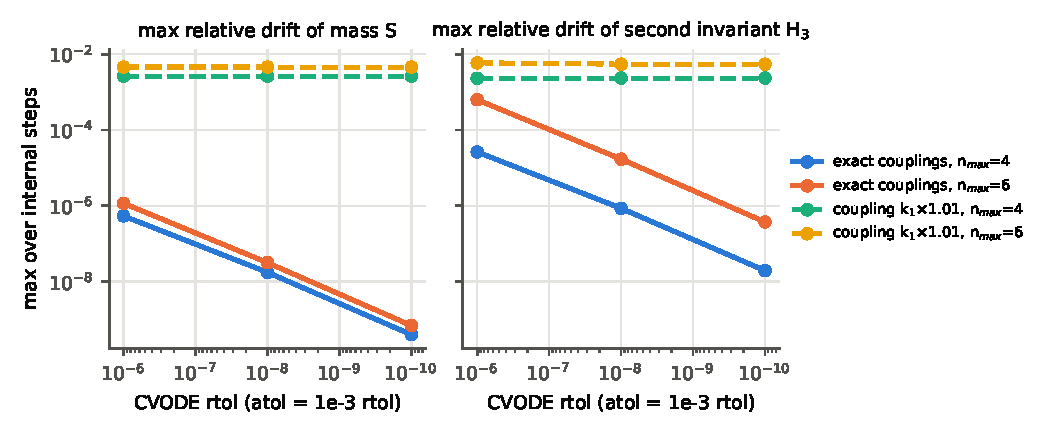
\includegraphics[width=0.6\linewidth]{data/fig_conservation_controls.pdf}
\caption{Drift against rtol for the positive control (converges) and the perturbed-coupling negative control (does not)
\tier{X}. Generated by \texttt{make\_figures.py} from \texttt{sigma3\_study.json}.}\label{fig:controls}
\end{figure}

\paragraph{Truncation sweep.} For $\sigma=3$, $n_{\max}=2..7$ and 2 phase seeds, $\sup_t2D\Omega(t)/(H_3(0)+S(0)^{3/2})$ lies
between $\SthreeMinRatio$ and $\SthreeMaxRatio$ with no trend in $N$. In \SthreeAboveTzero/\SthreeNruns{} runs the supremum
exceeds the $t=0$ value, so the dynamics move the ratio. The maximum drifts are $\SthreeMaxdS$ in $S$ and $\SthreeMaxdH$ in $H_3$
(Figure~\ref{fig:sweep}, left) \tier{X, SE-X-0002}.

\paragraph{$\sigma=2$ control (Table~\ref{tab:c2}).} On top-shell data ($v_{n_{\max}}=1$, other shells $10^{-3}$, $T=0.5$) the
$\sigma=2$ ratio grows from 0.667 to \CtwoTen. Its local $\log_2$ steps for $n_{\max}=6\to10$ are \CtwoLogSteps, in line with the
Remark's $D4^n/(D2^n+1)$. On this data the supremum equals the $t=0$ value to within a relative $\CtwoGapRel$ for
$\sigma=2$ (absolute $\CthreeGapAbs$ for $\sigma=3$), so the growth is static, not dynamical. On the same data
$\sigma=3$ reaches at most \CthreeMax{} and never exceeds 1. On cascading (decaying) data, $H_2$ is conserved to $\DecHtwoFour$
($n_{\max}=4$) and $\DecHtwoSix$ ($n_{\max}=6$), consistent with conservation for every $\omega$. Meanwhile the $\sigma=2$ enstrophy
grows to \DecOmegaFour{} and \DecOmegaSix, and the analogue ratio reaches \DecRatioFour{} and \DecRatioSix{} \tier{X, SE-X-0003}.

\begin{table}[h]\centering\small
\caption{Top-shell data, sup ratio $2D\Omega/(H_\sigma(0)+S(0)^{3/2})$, $D=\Dval$, rtol $10^{-10}$. ``supp.'' rows are
supplementary probes with the same binary and seeds (\texttt{sigma2\_probes.jsonl}).}\label{tab:c2}
\begin{tabular}{rrccl}\toprule
$n_{\max}$ & Lean $N$ & $\sigma=2$ & $\sigma=3$ & source\\\midrule
\tabinput{table_c2.tex}
\bottomrule\end{tabular}
\end{table}

\begin{figure}[h]\centering
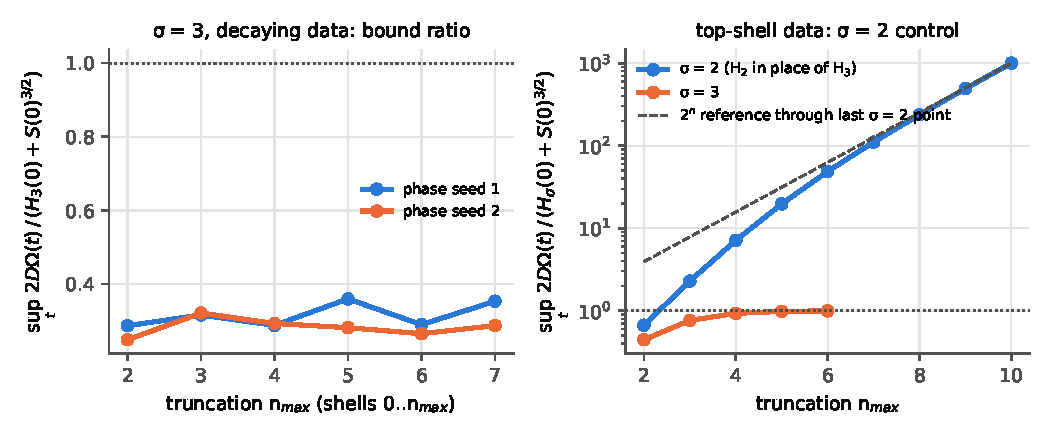
\includegraphics[width=0.85\linewidth]{data/fig_truncation_sweep.pdf}
\caption{Left: $\sigma=3$ bound ratio against truncation for decaying data. Right: top-shell data, $\sigma=2$ (grows like
$2^{n}$) against $\sigma=3$ ($\le1$). Dotted: the Lean bound, ratio $=1$ \tier{X}.}\label{fig:sweep}
\end{figure}

\section{HuggingFace dataset illustration}\label{sec:hf}

\paragraph{Dataset.} We use \texttt{polymathic-ai/turbulent\_radiative\_layer\_2D}, revision \hash{\WellRev}, licence CC-BY-4.0
per its card. It is part of The Well~\cite{thewell} and was generated with Athena++. It solves 2D compressible Euler with
radiative cooling, periodic in $x$ and zero-gradient in $y$, and its associated paper is~\cite{fielding} \tier{L, SE-L-0002}. We
downloaded one test file, \texttt{data/test/turbulent\_radiative\_layer\_tcool\_0.32.hdf5} (109\,MB, sha256
\hash{\WellHfiveSha}), and the card and YAML files.

\paragraph{What we computed.} For \WellNsnap{} developed snapshots (time indices 25, 50, 75, 100) we take the FFT of the velocity
along the periodic $x$ axis only, remove $k_x=0$, average over $y$, and sum $k_x\in[2^n,2^{n+1})$ into shells $n=0..5$. Pipeline
controls \WellControls. Parseval holds to $\WellParseval$, a synthetic $\sin(8x)$ field lands entirely in shell 3, and white noise
gives $\log_2$ slope \WellNoiseSlope. The data slopes are \WellSlopes. The moduli, normalised to $S=1$ with 2 random phase
seeds, initialise \WNruns{} $\sigma=3$ runs ($n_{\max}=5,6,7$, upper shells zero). The bound holds in all of them, with
maximum ratio \WMaxRatio. The supremum exceeds the $t=0$ value in \WAbove/\WNruns. Drifts are $\le\WMaxdS$ in $S$ and $\le\WMaxdH$ in $H_3$
(Figure~\ref{fig:well}) \tier{X, SE-X-0004}.

\paragraph{Caveats.} The data provide a realistic spectral shape, nothing more. The flow is compressible and cooling, and does not
conserve energy. The spectrum is 1D, uses velocity only (not $\sqrt\rho\,u$) and carries no phases. The phases are random. Over
$T=2$ the zero-initialised top shells barely fill, so the ratio is the same at $n_{\max}=5,6,7$ and these runs do not probe cutoff
dependence.

\begin{figure}[h]\centering
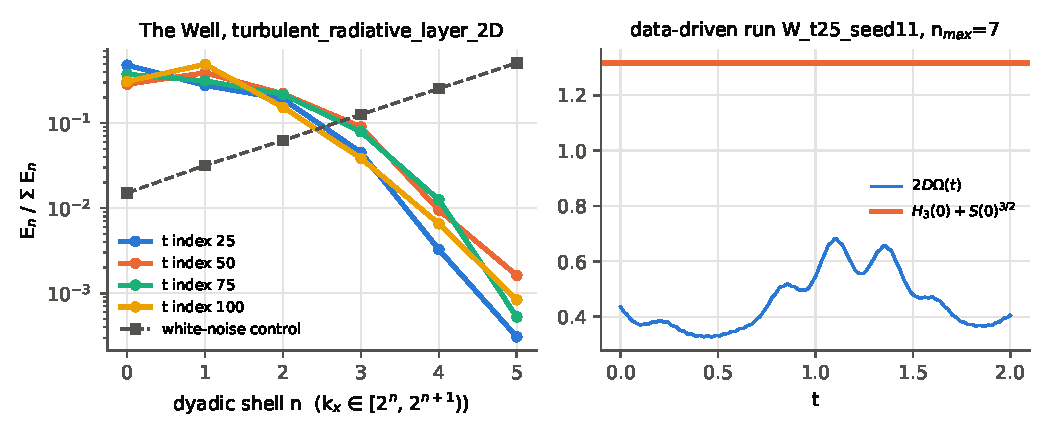
\includegraphics[width=0.85\linewidth]{data/fig_well_data.pdf}
\caption{Left: dyadic shell spectra of The Well snapshots and a white-noise control. Right: one data-initialised run,
$2D\Omega(t)$ against the Lean bound \tier{X}.}\label{fig:well}
\end{figure}

\section{Limitations}\label{sec:limits}
\begin{itemize}\itemsep1pt
\item \emph{Verification.} The producer checked the files, another AI agent instance recompiled them at paper stage, and a
separate AI-agent instance ran an independent audit (\texttt{AUDIT.md}). It recompiled the claimed and prior files (rc 0, every
audited declaration within the allowlist), planted its own \lean{sorry} and axiom and saw the axiom audit flag exactly the
dependent theorems, checked statement fidelity against \lean{\#print} of the owner definitions, and reran the numerics and
tests. No human has audited statement adequacy (all Tier~A ledger rows carry \texttt{audit: null}).
\item \emph{Solution hypothesis.} Existence is assumed. The hypothesis uses two-sided \lean{HasDerivAt} at every
$t\in[0,T]$, endpoints included. For $T<0$ the interval is empty and the along-flow statements are vacuous. The zero trajectory satisfies it (\lean{zero\_trajectory\_is\_solution}); this shows consistency,
not non-triviality.
\item \emph{Fixed $N$.} There is no infinite-shell statement. Cutoff uniformity needs $N$-uniform $\Omega(0)$ and $S(0)$
(Corollary~\ref{cor:omega}, Tier~C).
\item \emph{Definitions.} The model is the owner's conjugated complexification plus dispersion. Its physical fidelity is the
owner's design choice and is not certified here.
\item \emph{Numerics.} $n_{\max}\le7$, a single $D$, finite $T$, suprema at step points. The BDF damping of fast rotations gives a
negative $S$ drift (largest $-2.8\times10^{-5}$ for $\sigma=3$ top-shell data at $n_{\max}=6$, $-1.3\times10^{-4}$ for $\sigma=2$ at
$n_{\max}=10$). Damping lowers $\Omega$ and so biases runs toward passing, but it cannot explain the passes. In the sweep and the
data runs the margin to the bound is at least $1-\WMaxRatio$, far above the drifts. For the top-shell $\sigma=3$ runs (up to
$\CthreeMax$) the supremum exceeds the $t=0$ value by at most $\CthreeGapAbs$, far below the margin $1-\CthreeMax$ to the
bound. Larger $N$ would need an exponential or
splitting integrator, which was not attempted.
\item \emph{Scope.} The open second half of the memo's step (the ``O5 trap'' argument) was not attempted. No novelty is claimed
for the inequality, which is a corollary of the owner's lemma. A literature check on complex dyadic and SHG-chain models,
listed as pending in the memo, was not completed here.
\end{itemize}

\section{Reproducibility}\label{sec:repro}
Lean (from the AutoevolveAI worktree; \texttt{OUT.json} is any output path):
\begin{lstlisting}[language={}]
taskset -c 4-7 .venv/bin/python -I results/autoresearch/2026-10-25/H7/contribution/run_lean.py \
  results/autoresearch/2026-10-25/H7/contribution/Autoresearch_EnstrophyFlow.lean OUT.json
python -I results/autoresearch/2026-10-25/H7/contribution/paper_stage_recompile.py
\end{lstlisting}
Rust: rusty-SUNDIALS worktree, branch \texttt{physics/ar-sigma3-shell-2026-10-25}, based on origin/main
\hash{47ef5044c10b04c64d8c86f483f1aa47c400ab28}. Code commit \hash{99f5df89e8d8380ea1a9f065ae87308e779224fc}, results
\hash{e869e5fc4e38df24bc93ee2c22e19f2e68920041}, $\sigma=2$ probes \hash{dfa9a0880450a7601e1ecdcb735b5897c6319ffd}.
These commits are not pushed at the time of writing.
\begin{lstlisting}[language={}]
CARGO_TARGET_DIR=/home/callensxavier_gmail_com/rusty-target-ar cargo test --release -j 2 --offline \
  --manifest-path WT/Cargo.toml -p qf-shell-cascade -- --test-threads=2
venv-pta/bin/python -I R/scripts/well_spectrum.py \
  hf-data/sigma3_enstrophy/data/test/turbulent_radiative_layer_tcool_0.32.hdf5 R/well_spectrum.json   # needs h5py
python -I R/scripts/make_amps.py R/well_spectrum.json R/well_amps.txt
taskset -c 4-7 /home/callensxavier_gmail_com/rusty-target-ar/release/sigma3_study full R/sigma3_study.json \
  R/well_amps.txt 99f5df89e8d8380ea1a9f065ae87308e779224fc
python -I R/scripts/run_probes.py /home/callensxavier_gmail_com/rusty-target-ar/release/sigma3_study R/sigma2_probes.jsonl
python -I R/scripts/summarise.py R/sigma3_study.json R/summary.json
python -I R/scripts/make_figures.py R/sigma3_study.json R/well_spectrum.json R/figures R/sigma2_probes.jsonl
\end{lstlisting}
Here \texttt{WT} is the rusty-SUNDIALS worktree and \texttt{R} is \texttt{WT/crates/qf-shell-cascade/results/sigma3}. Absolute
paths are in \texttt{H7/contribution/NUMERICS.md}. Paper:
\texttt{python -I gen\_numbers.py; python -I make\_listings.py; pdflatex main.tex} (twice);
ledger: \texttt{python -I ledger/build\_ledger.py}.

\section{Claim ledger}\label{sec:ledger}
\texttt{ledger/ledger.json} holds 7 Tier~A, 2 Tier~L, 4 Tier~C and 5 Tier~X rows. Each row points to a
content-addressed evidence blob in \texttt{ledger/evidence/}. Tier~A blobs hold verbatim axiom lines with source and
\texttt{.olean} hashes. Tier~L blobs hold the excerpts, Tier~C blobs the argument, and Tier~X blobs the result-file hashes
with \texttt{claim\_licence: false}. The Elenchus gate (\texttt{tools/ledger.py ledger.json --evidence-dir evidence}) was
run on it. Its output is in \texttt{ledger/gate\_output.txt}: exit code 1, no blocking findings, and one
\texttt{LEDGER\_UNAUDITED\_TIER\_A} flag per Tier~A row, because no person has audited statement adequacy. The Waleffe
Theorem~1 source text used by the auditor's Elenchus \texttt{citation\_check.py} run is persisted in \texttt{ledger/sources/}
with its claim file; the rerun there returns ACCEPTED (exit 0, tier ceiling L), recorded in
\texttt{ledger/sources/citation\_check\_output.txt}.

\begin{thebibliography}{9}\small
\bibitem{qfrepo} SocrateAI-Scientific-QuantumFluids, project repository (owner's Lean sources \texttt{lean\_src/QuantumFluidsShell.lean},
\texttt{lean\_src/ShellHamiltonian.lean}, design memo \texttt{docs/DUAL\_SCALE\_PROPOSAL.md} \S5, \S7), commit
\hash{10f74daf1b39d2ac51a785452329fff0003cfc83}. Project document, not peer reviewed.
\bibitem{waleffe} F.~Waleffe, \emph{On some dyadic models of the Euler equations}, arXiv:math/0410380 (2004).
\bibitem{thewell} R.~Ohana, M.~McCabe, et al., \emph{The Well: a Large-Scale Collection of Diverse Physics Simulations for
Machine Learning}, arXiv:2412.00568 (2024).
\bibitem{fielding} D.~B.~Fielding, E.~C.~Ostriker, G.~L.~Bryan, A.~S.~Jermyn, \emph{Multiphase gas and the fractal nature of
radiative turbulent mixing layers}, Astrophys.\ J.\ Lett.\ 894, L24 (2020), doi:10.3847/2041-8213/ab8d2c (as given in the dataset card; not read by us).
\bibitem{sundials} D.~J.~Gardner, D.~R.~Reynolds, C.~S.~Woodward, C.~J.~Balos, \emph{Enabling New Flexibility in the SUNDIALS Suite of Nonlinear and
Differential/Algebraic Equation Solvers}, ACM Trans.\ Math.\ Softw., arXiv:2011.10073 (2020) (authors, title and
identifier verified; cited for the
SUNDIALS/CVODE design only).
\bibitem{rusty} rusty-SUNDIALS, Rust workspace re-implementing SUNDIALS integrators; branch and commits as in
Section~\ref{sec:repro}.
\bibitem{uotiered} X.~Callens, \emph{Planar universal optimality, tiered: kernel-checked consequences, a non-uniqueness
theorem, and a CVODE N-body consistency check for the Yukawa interaction}, v2, doi:10.5281/zenodo.23293429; cited for the
tiering and ledger method.
\bibitem{uotextbook} X.~Callens, student textbook on triangular-lattice universal optimality (2026),
doi:10.5281/zenodo.23295142; cited for the tiering method.
\end{thebibliography}
\end{document}
